% Evans 4.5.1--2, printed pp. 200--206; PDF pp. 217--223.
\Needspace{65mm}
\section{Asymptotics}\label{sec:4-5}
The source presents several asymptotic constructions formally.
We distinguish exact algebraic identities, proved local integral
asymptotics, and conditional PDE expansions.
No convergence theorem is inferred merely by matching powers.

\Needspace{35mm}
\subsection{A small-diffusion plume: geometry and transverse scale}
Consider $\operatorname{div}(\mathbf b\,\mu)=\delta_0$ in two dimensions.
Let $\dot X=\mathbf b(X)$, $X(0)=0$, and suppose $|\mathbf b(X)|>0$.
If the forward trajectory leaves compact sets, the locally finite measure
\[
 \int\phi\,d\mu=\int_0^\infty\phi(X(t))\,dt
\]
solves this equation, since
\[
 -\int\mathbf b\cdot D\phi\,d\mu
 =-\int_0^\infty\frac d{dt}\phi(X(t))\,dt=\phi(0).
\]
This is an outgoing solution; an extra background homogeneous solution
is not excluded by this calculation.
With speed $\sigma=|\mathbf b(X)|$, tangent $\tau$ and unit normal $\nu$,
use $x=X(t)+y\nu(t)$ in a nonoverlapping tubular neighborhood.
Frenet identities give $\nu'=-\sigma\kappa\tau$ and
\[
 x_t=\sigma(1-\kappa y)\tau,\quad x_y=\nu,\quad
 dx=H\,dt\,dy,\qquad H=\sigma(1-\kappa y)>0.
\]
Thus the same measure has density $\delta(y)/\sigma(t)$ with respect
to spatial area.
\Needspace{45mm}
\PDEAnnotation{线上的密度必须带速度因子}{注入量按行进时间计量，而面积元在曲线处含 $\sigma(t)$。因此横向 Dirac 前要乘 $1/\sigma$。若轨道封闭或反复回返，时间积分可能不是局部有限测度。}

Now perturb to $-\varepsilon\Delta u^\varepsilon+
\operatorname{div}(\mathbf b u^\varepsilon)=\delta_0$.
Away from the injection point, set
$z=y/\sqrt\varepsilon$,
$u^\varepsilon=\varepsilon^{-1/2}v^\varepsilon(t,z)$.
The coordinate metric gives the exact identity
\[
 \Delta w=\frac1H\partial_t(H^{-1}w_t)
                  +\frac1H\partial_y(Hw_y).
\]
Also write
$\mathbf b=(\sigma+\alpha y+O(y^2))\tau+
(\beta y+O(y^2))\nu$.
Then on compact $t>0$, bounded $z$, provided the needed derivatives
of $v^\varepsilon$ are uniformly bounded,
\[
 \mathbf b\cdot Dv^\varepsilon
       =v^\varepsilon_t+\beta z v^\varepsilon_z+O(\sqrt\varepsilon),
 \qquad
 \varepsilon\Delta v^\varepsilon=v^\varepsilon_{zz}+O(\sqrt\varepsilon),
\]
\[
 \operatorname{div}\mathbf b
       =\sigma'/\sigma+\beta+O(\sqrt\varepsilon).
\]
For example the transverse first-derivative term in the Laplacian
is $\varepsilon(H_y/H)\partial_yv^\varepsilon=O(\sqrt\varepsilon)$;
the tangential second-derivative terms are $O(\varepsilon)$.
Thus the conditional leading equation is
\[
 v_t-v_{zz}+(\beta z v)_z+(\sigma'/\sigma)v=0,\qquad
 v(0)=\delta_0/\sigma(0).
 \tag{PL4}
\]
Its exact Gaussian solution, derived again in Problem 13, is
\[
 v(t,z)=\frac{e^{-z^2/\Gamma(t)}}{\sigma(t)\sqrt{\pi\Gamma(t)}},
 \qquad \Gamma'=4+2\beta\Gamma,\quad\Gamma(0)=0 .
\]
Indeed $A=\sigma v$ satisfies $A_t=A_{zz}-(\beta zA)_z$;
substituting the Gaussian gives the displayed ODE and mass $\int A=1$.
The transverse width is $\sqrt{\varepsilon\Gamma(t)}$.
This does not by itself prove approximation of the original elliptic
Green function, nor control the injection region or large times.
\Needspace{45mm}
\PDEAnnotation{形式余项依赖尚未证明的统一界}{把 $y$ 换成 $\sqrt\varepsilon z$ 后，系数误差很小，但它仍乘着解的导数。只有这些导数在所考察区域有统一界，才能写成统一的 $O(\sqrt\varepsilon)$。}

\Needspace{35mm}
\subsection{Laplace concentration and vanishing viscosity}\label{sec:4-laplace}
\begin{lemma}[Source asymptotics lemma, with tail control]
Let $k,l$ be continuous on $\R$, $|l(y)|\leq C(1+|y|)$,
and $k(y)\geq c y^2-C$, $c>0$.
If $k$ has a unique minimum at $y_0$, then
\[
 \frac{\int l(y)e^{-k(y)/\varepsilon}\,dy}
      {\int e^{-k(y)/\varepsilon}\,dy}\longrightarrow l(y_0).
 \tag{LC4}
\]
\end{lemma}
\begin{expandedproof}
Subtract the minimum $k_0$ and put $h=k-k_0\geq0$.
Fix a small neighborhood $N$ of $y_0$ on which
$|l-l(y_0)|<\eta$.
On a large compact interval outside $N$, $h\geq d>0$ by uniqueness.
Increase the interval so that outside it
$h(y)\geq d/2+(c/2)y^2$, decreasing $d$ if necessary.
By continuity there is an interval of length $2r>0$ near $y_0$
where $h<d/4$.
The denominator is at least $2r e^{-d/(4\varepsilon)}$.
The numerator of the absolute error over the compact complement
is at most $C_1e^{-d/\varepsilon}$.
The tail numerator is bounded by
\[
 C_2e^{-d/(2\varepsilon)}
       \int(1+|y|)e^{-cy^2/(2\varepsilon)}\,dy,
\]
whose ratio to the denominator tends to zero.
Inside $N$ the normalized error is at most $\eta$.
Let $\varepsilon\downarrow0$ and then $\eta\downarrow0$.
This proves concentration together with the required control of
the unbounded observable $l$.
\end{expandedproof}
\Needspace{45mm}
\PDEAnnotation{逐点密度趋零不足以推出集中}{归一化密度在每个非极小点趋零，还不能控制积分或无穷远的质量。证明需要分母下界、远离极小点的能量间隙，以及带权尾积分。}

For bounded initial $g$, let $P'=g$ and
$K(y)=(x-y)^2/(2t)+P(y)$.
The quadratic term dominates the Lipschitz primitive.
Formula (VB4) and (LC4), with parameter $2\varepsilon$, imply
\[
 u^\varepsilon(x,t)\longrightarrow \frac{x-y(x,t)}t
\]
whenever the minimizing point is unique.
By Chapter~3, at each $t>0$ only countably many $x$ have multiple
minimizers, and the right side is the Lax--Oleinik entropy solution.
Since $|u^\varepsilon|\leq\|g\|_\infty$, this convergence is also
$L^1_{\rm loc}$ in $x$ for each fixed $t$.
Joint a.e. convergence and the same bound give local space-time
$L^1$ convergence away from zero.
The multiple-minimizer set is measurable, for instance by expressing
separation of two minimizers using rational compact neighborhoods;
Fubini therefore applies to the countable time slices.
\Needspace{45mm}
\PDEAnnotation{与第三章的最小化公式接上了}{黏性解是最优速度的指数加权平均。黏性趋零时，权重集中到作用量最低点；最低点的分支竞争正对应守恒律的激波。}

If $k$ is smooth with finitely many nondegenerate global minima $y_j$,
local Taylor expansion $y=y_j+\sqrt\varepsilon z$ and Gaussian
domination give
\[
 \int l e^{-k/\varepsilon}
 =e^{-k_0/\varepsilon}\sqrt{2\pi\varepsilon}
       \left(\sum_j\frac{l(y_j)}{\sqrt{k''(y_j)}}+o(1)\right).
\]
To justify domination, restrict to a small neighborhood where
$k-k_0\geq c_j|y-y_j|^2$, and use the energy gap outside.
Thus at a tie the limit is a weighted average, not necessarily
the velocity at one selected minimizing point.
Values on shock curves do not affect the weak solution.
% Supplement to Evans 4.5.3, printed pp. 207--217.
\Needspace{35mm}
\subsection{Geometric optics and stationary phase}\label{sec:4-stationary}
For $u^\varepsilon=a e^{ip/\varepsilon}$ the exact wave-operator identity is
\[
 \begin{aligned}
 &e^{-ip/\varepsilon}(u^\varepsilon_{tt}-\Delta u^\varepsilon)\\
 &\quad=\varepsilon^{-2}a(|Dp|^2-p_t^2)\\
 &\qquad+\frac{i}{\varepsilon}
       \{2p_ta_t-2Dp\cdot Da+a(p_{tt}-\Delta p)\}
       +(a_{tt}-\Delta a).
 \end{aligned}
\]
Matching the first two orders gives the eikonal and amplitude equations
\[
 p_t^2=|Dp|^2,\qquad
 2p_ta_t-2Dp\cdot Da+(p_{tt}-\Delta p)a=0 .
\]
On a smooth nonzero-frequency branch choose $p_t=\pm|Dp|$.
The sign cannot be chosen independently at every point.
For $u_{tt}-\sum a_{ij}(x)u_{x_ix_j}=0$ the first equation becomes
$p_t^2=\sum a_{ij}p_{x_i}p_{x_j}$, with the corresponding amplitude
expression obtained by the same differentiation.
These identities define a candidate expansion.
A theorem about exact solutions needs control of the residual and
the evolution, especially near caustics.
\Needspace{45mm}
\PDEAnnotation{相位误差除以小参数会放大}{即使 $p^\varepsilon-p=o(1)$，也不能直接推出两个指数相近；指数里的差是 $(p^\varepsilon-p)/\varepsilon$。振荡展开需要比普通逐点收敛更精确的误差尺度。}

\begin{lemma}[Nonstationary phase; strengthening source Lemma 1]
If $a\in C_c^\infty$ and $|D\phi|>0$ on its support, then for every
integer $N\geq1$,
$\int e^{i\phi/\varepsilon}a=O(\varepsilon^N)$.
\end{lemma}
\begin{expandedproof}
Near the support let $V=D\phi/|D\phi|^2$.
Then $V\cdot D e^{i\phi/\varepsilon}=(i/\varepsilon)e^{i\phi/\varepsilon}$.
Integration by parts gives
\[
 \int e^{i\phi/\varepsilon}a
 =-\frac{\varepsilon}{i}\int e^{i\phi/\varepsilon}
                                  \operatorname{div}(aV).
\]
Iterate $N$ times; the final smooth compactly supported amplitude
has finite $L^1$ norm independent of $\varepsilon$.
This also proves the source's linear-phase case.
\end{expandedproof}

\begin{lemma}[Quadratic phase; source Lemma 2]
For real symmetric invertible $H$ and $a\in C_c^\infty(\R^d)$,
\[
 \int e^{iz\cdot Hz/(2\varepsilon)}a(z)\,dz
 =(2\pi\varepsilon)^{d/2}
   \frac{e^{i\pi\operatorname{sgn}H/4}}{|\det H|^{1/2}}
      [a(0)+O(\varepsilon)].
 \tag{QP4}
\]
\end{lemma}
\begin{expandedproof}[regularization, branch and error]
For $\operatorname{Re}q>0$,
\[
 \int_{\R} e^{-qs^2+ibs}\,ds=\sqrt{\pi}\,q^{-1/2}e^{-b^2/(4q)} .
\]
Choose the square root with positive real part.
For real positive $q$ this is the Gaussian identity; analytic
continuation in the right half-plane proves it for complex $q$,
since compact subsets admit an integrable Gaussian majorant.
Equivalently the contour argument of Problem 15 proves it directly.

Diagonalize $H$ orthogonally, multiply the phase by
$e^{-\eta|z|^2}$, and apply this identity in each coordinate.
As $\eta\downarrow0$, an eigenvalue $\lambda$ contributes the factor
$|\lambda|^{-1/2}e^{i\pi\operatorname{sgn}\lambda/4}$ after the common
$(2\pi\varepsilon)^{1/2}$ factor.
Insert Fourier inversion for $a$ before this calculation.
Its transform is rapidly decreasing.
The regularized Gaussian integral is uniformly bounded in frequency,
so dominated convergence yields the exact oscillatory identity
\[
 \begin{aligned}
 \int e^{iz\cdot Hz/(2\varepsilon)}a(z)\,dz
 &=C_{\varepsilon,H}(2\pi)^{-d/2}\\
 &\quad\cdot\int \widehat a(\xi)
                e^{-i\varepsilon\xi\cdot H^{-1}\xi/2}\,d\xi ,
 \end{aligned}
\]
where $C_{\varepsilon,H}$ is the prefactor in (QP4).
Since $|e^{ir}-1|\leq|r|$, the bracket differs from $a(0)$ by at most
\[
 C\varepsilon\int |\xi|^2|\widehat a(\xi)|\,d\xi<\infty .
\]
This proves both the constant and the error in (QP4).
\end{expandedproof}

\begin{lemma}[Morse coordinates; source Lemma 3(ii)]
If $D\phi(0)=0$ and $H=D^2\phi(0)$ is invertible, there is a local
smooth diffeomorphism $\Phi$ with $\Phi(0)=0$, $D\Phi(0)=I$, and
$\phi(\Phi(z))=\phi(0)+z\cdot Hz/2$.
\end{lemma}
\begin{expandedproof}[an editorial matrix proof]
Taylor's formula with integral remainder gives
$\phi(x)=\phi(0)+x^TA(x)x/2$, where
$A(x)=2\int_0^1(1-s)D^2\phi(sx)\,ds$ and $A(0)=H$.
On symmetric matrices solve
\[
 H+2S+SH^{-1}S=A(x).
\]
The derivative in $S$ at zero is $2I$, so the implicit function
theorem gives a smooth symmetric $S(x)$ with $S(0)=0$.
Set $B=I+H^{-1}S$; then $B^THB=A$.
The map $z=B(x)x$ has derivative $I$ at zero.
Its local inverse $\Phi$ has the required properties.
This works for indefinite $H$ as well as positive definite $H$.
\end{expandedproof}
For completeness the source's noncritical coordinate lemma is also
elementary. Choose rows $r_1,\ldots,r_{d-1}$ complementary to
$D\phi(0)$, impose $r_j\cdot(y-x)=0$ and
$\phi(y)-\phi(0)=D\phi(0)\cdot x$.
The $y$ Jacobian is invertible; the implicit function theorem
gives $y=\Phi(x)$ and differentiation gives $D\Phi(0)=I$.


\PDEBodyDiagram{4.4}{Near a nondegenerate stationary point the scale is square-root.}
{For phase $x^2$, oscillation is slow near its stationary point at zero and rapid farther away. The highlighted interval has width $2\sqrt{\varepsilon}$. Rescaling $x=\sqrt{\varepsilon}\,z$ explains the leading $\varepsilon^{1/2}$ factor in one dimension; cancellation, not pointwise smallness of the integrand, suppresses the outer region.}
{ch04-stationary-window}

\begin{theorem}[Nondegenerate stationary phase]
Suppose $\phi$ has just finitely many critical points $z_j$ on
$\operatorname{supp}a$, and all $H_j=D^2\phi(z_j)$ are invertible.
Then
\[
 \int e^{i\phi(z)/\varepsilon}a(z)\,dz
 =(2\pi\varepsilon)^{d/2}
 \sum_j\frac{e^{i\phi(z_j)/\varepsilon+i\pi\operatorname{sgn}H_j/4}}
                 {|\det H_j|^{1/2}}
                  [a(z_j)+O(\varepsilon)].
 \tag{SP4}
\]
\end{theorem}
\begin{expandedproof}
Choose a partition of unity separating small neighborhoods of the
critical points from the noncritical compact remainder.
The latter is $O(\varepsilon^N)$ for arbitrary $N$ by the first lemma.
At each critical point change to Morse coordinates.
The transformed amplitude is $a(\Phi(z))|\det D\Phi(z)|$
times its cutoff and equals $a(z_j)$ at the origin.
Apply (QP4) to each localized integral and add them.
Taking $N>d/2+1$ absorbs the noncritical remainder.
\end{expandedproof}
\Needspace{45mm}
\PDEAnnotation{行列式为零时不能继续用驻相公式}{$|\det H|^{-1/2}$ 描述非退化临界点的集中强度。它发散时，表示这一阶近似失效；需研究更高阶相位，不能把发散系数直接当作精确解的无穷大。}

\paragraph{Recovering the rays of Chapter 3.}
For high-frequency displacement $g^\varepsilon(z)=a(z)e^{ip_0(z)/\varepsilon}$
with $|Dp_0|>0$ on $\operatorname{supp}a$ and zero initial velocity,
Fourier representation splits the wave into two equal half-waves.
After frequency rescaling their phases are
\[
 \phi_\pm(x,y,z,t)=(x-z)\cdot y\pm t|y|+p_0(z).
\]
The critical equations are
\[
 y=Dp_0(z),\qquad x=z\mp t\,\frac{Dp_0(z)}{|Dp_0(z)|}.
 \tag{RAY4}
\]
These are exactly the projected HJ rays for $p_t\mp|Dp|=0$.
The joint Hessian at a critical point is
\[
 \begin{pmatrix}
 \displaystyle\pm\frac t{|y|}(I-\widehat y\otimes\widehat y)&-I\\
 -I&D^2p_0(z)
 \end{pmatrix},\qquad \widehat y=y/|y|.
\]
Its determinant equals $(-1)^n$ times the Jacobian determinant
of the ray map in (RAY4), by block elimination.
For small time that map is locally invertible.
The critical value is $p_0(z)$, since
$(x-z)\cdot y\pm t|y|=0$.
Applying (SP4) in $2n$ variables cancels the half-wave prefactor
$(2\pi\varepsilon)^{-n}$ and gives the amplitude
$a(z)/|\det D_zx|^{1/2}$ and the Hessian signature phase.
The two half-waves are then added with weight $1/2$.

The amplitude in $y,z$ is initially not compact in $y$.
To justify this application, first cut frequencies off to a compact
neighborhood of $Dp_0(\operatorname{supp}a)$ disjoint from zero.
Outside that neighborhood $D_z\phi=Dp_0-y$ is nonzero.
Repeated integration by parts in $z$ makes the tail integrable in
$y$, with arbitrarily high powers of $\varepsilon$; for large $y$
each integration also supplies inverse powers of $|y|$.
This reduces to the compactly supported theorem.
The formula is local before caustics or summed over the finitely many
nondegenerate preimages; it asserts no uniform approximation at a caustic.
\par\noindent\begin{minipage}{\linewidth}
\begin{center}
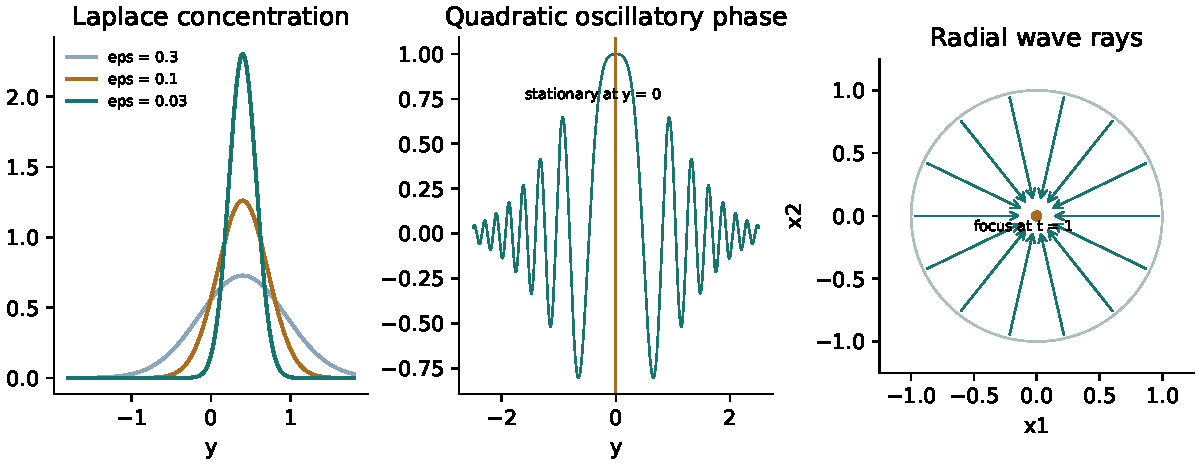
\includegraphics[width=\linewidth]{output/figures/ch04-concentration-rays.pdf}
\end{center}
\noindent\emph{Editorial figure.} Laplace concentration is compared
with oscillatory cancellation; the ray diagram displays a focusing map
whose Jacobian eventually vanishes.
\end{minipage}

% Supplement to Evans 4.5.4, printed pp. 217--220.
\Needspace{35mm}
\subsection{Periodic homogenization: expansion, cell problem, and a proof}
\label{sec:4-homogenization}
We use the symmetric uniformly elliptic case, sufficient also for
Problem 18: $A(y)=A(y)^T$ is smooth, $Q$-periodic,
$Q=(0,1)^n$, and $\theta I\leq A\leq\Theta I$.
Consider $-\operatorname{div}(A(x/\varepsilon)Du^\varepsilon)=f$
on a bounded Lipschitz domain with zero trace and $f\in L^2$.
The source uses a formal expansion; we first derive it, then give
a weak-convergence proof under these stated hypotheses.

\paragraph{Two-scale bookkeeping.}
Write $u^\varepsilon=u_0(x,y)+\varepsilon u_1(x,y)+\cdots$,
$y=x/\varepsilon$, with all $u_j$ periodic in $y$.
Every spatial derivative becomes $D_x+\varepsilon^{-1}D_y$.
Thus the three operator pieces are
\[
 L_1=-D_y\cdot AD_y,\quad
 L_2=-D_y\cdot AD_x-D_x\cdot AD_y,\quad
 L_3=-D_x\cdot AD_x .
\]
The coefficients of $\varepsilon^{-2},\varepsilon^{-1},1$ give
\[
 L_1u_0=0,\quad L_1u_1+L_2u_0=0,\quad
 L_1u_2+L_2u_1+L_3u_0=f .
\]
Testing the first identity by $u_0$ and integrating over $Q$ gives
$D_yu_0=0$; opposite periodic faces cancel.
For zero-mean correctors $\chi_i$, define
\[
 \operatorname{div}_y\{A(y)(e_i-D_y\chi_i)\}=0,\qquad
 \int_Q\chi_i=0 .
 \tag{CELL4}
\]
Then $u_1=-\sum_i\chi_i(y)u_{x_i}$ solves the next equation.
Averaging the order-one equation kills $L_1u_2$ and yields
\[
 -\operatorname{div}(\overline A Du)=f,\qquad
 \overline A e_i=\int_Q A(y)(e_i-D\chi_i)\,dy .
 \tag{HOM4}
\]
The minus sign in $u_1$ matches the source's corrector convention.
Many other texts use $\varphi_i=-\chi_i$ and a plus sign instead.

\Needspace{45mm}
\PDEAnnotation{平均的是修正后的通量}{有效系数通常不是直接对 $A$ 求平均。微观梯度要先调整成 $e_i-D\chi_i$，使通量在单元中无散，再取平均；一维时结果是调和平均而非算术平均。}

\PDEMarginDiagram{4.M}{一维有效系数}
{两个半格串联时通量相同，梯度与系数成反比。平均的是阻力 $1/a$，再取倒数。分段常系数可按弱形式理解。}
{ch04-cell-margin}

\begin{lemma}[Cell solvability and effective ellipticity]
(CELL4) has a unique zero-mean periodic weak solution.
The matrix $\overline A$ is symmetric and satisfies
$\theta I\leq\overline A\leq\Theta I$.
\end{lemma}
\begin{expandedproof}
On the zero-mean periodic $H^1$ space minimize
$\int_Q(e_i-Dv)\cdot A(e_i-Dv)$.
Periodic Poincar\'e and ellipticity bound every minimizing sequence
in $H^1$; weak compactness and weak lower semicontinuity give a minimizer.
The first variation is
$\int_Q A(D\chi_i-e_i)\cdot D\psi=0$.
Strict convexity in the gradient makes the difference of two
minimizers constant, hence zero after normalization.
These are standard Hilbert-space compactness and periodic Poincar\'e
facts; the cell equation is not solved merely by asserting zero mean.

For $\xi\in\R^n$, let $\chi_\xi=\sum_i\xi_i\chi_i$.
The cell identity allows any gradient $D\chi_\eta$ to be subtracted
from the other factor, so
\[
 \eta\cdot\overline A\xi
 =\int_Q(\eta-D\chi_\eta)\cdot A(\xi-D\chi_\xi).
\]
This proves symmetry.
The minimum over all periodic $v$ equals
$\xi\cdot\overline A\xi$ by orthogonality.
Its lower bound is
$\theta\int_Q|\xi-Dv|^2\geq\theta|\xi|^2$,
since $\int_QDv=0$ and $|Q|=1$.
The competitor $v=0$ gives the upper bound.
\end{expandedproof}

\begin{theorem}[An editorial rigorous homogenization statement]
Under the symmetric hypotheses above,
$u^\varepsilon\rightharpoonup u$ in $H_0^1$ and
$u^\varepsilon\to u$ in $L^2$, where $u$ is the unique weak solution of (HOM4).
\end{theorem}
\begin{expandedproof}[oscillating tests replace an unproved expansion]
Testing the original PDE by $u^\varepsilon$ gives a uniform $H_0^1$
bound by ellipticity and Poincar\'e.
Take a weakly convergent subsequence and use Rellich for strong $L^2$
convergence. The fluxes
$\eta^\varepsilon=A(x/\varepsilon)Du^\varepsilon$
are bounded in $L^2$; take a weak limit $\eta$.
The PDE gives $-\operatorname{div}\eta=f$.

For each $i$ put
\[
 w_i^\varepsilon=x_i-\varepsilon\chi_i(x/\varepsilon),\qquad
 q_i^\varepsilon=A(x/\varepsilon)Dw_i^\varepsilon .
\]
Periodic averaging implies $w_i^\varepsilon\to x_i$ in $L^2_{\rm loc}$
and $q_i^\varepsilon\rightharpoonup\overline A e_i$ in $L^2_{\rm loc}$;
also $\operatorname{div}q_i^\varepsilon=0$.
The averaging fact follows first by summing integrals on full
$\varepsilon$-cells for continuous periodic functions and compact tests,
then by $L^2(Q)$ approximation and uniform local cell bounds.

For $\phi\in C_c^\infty(U)$ symmetry gives
$\eta^\varepsilon\cdot Dw_i^\varepsilon
=Du^\varepsilon\cdot q_i^\varepsilon$.
Integrate the two sides by parts in different ways:
\[
 \int\phi\,\eta^\varepsilon\cdot Dw_i^\varepsilon
 =\int f\phi w_i^\varepsilon-\int w_i^\varepsilon\eta^\varepsilon\cdot D\phi,
\]
\[
 \int\phi\,Du^\varepsilon\cdot q_i^\varepsilon
 =-\int u^\varepsilon q_i^\varepsilon\cdot D\phi .
\]
Every product in these two right sides has a strong $L^2$ factor
and a weak $L^2$ factor.
The limits give $\eta_i=Du\cdot\overline A e_i$.
By symmetry this says $\eta=\overline A Du$, proving (HOM4).
Effective ellipticity gives uniqueness, so every subsequence has the
same limit; the entire family converges.
\end{expandedproof}
\Needspace{45mm}
\PDEAnnotation{两个弱收敛量不能直接相乘}{$A(x/\varepsilon)$ 与 $Du^\varepsilon$ 都会振荡，不能分别取弱极限再相乘。振荡测试把乘积改写为一个强收敛因子和一个弱收敛因子的配对，才识别出有效通量。}
The expansion need not satisfy the original boundary condition termwise;
boundary layers may be necessary for a quantitative error estimate.
We have proved weak $H^1$ convergence, not strong convergence of
the gradients or an $O(\varepsilon)$ global error.
For nonsymmetric coefficients the source's formal cell calculation
still applies with consistent index orientation; the rigorous testing
argument uses adjoint correctors. That extension is not asserted here.